\documentclass[11pt,a4paper]{article}

\usepackage[utf8]{inputenc}
\usepackage{graphicx}
\usepackage{float}
\usepackage{aeguill}
\usepackage{titlesec}
\usepackage[singlespacing]{setspace}
\usepackage[left=2.5cm,right=2.5cm,top=2cm,bottom=2cm]{geometry}

\setlength{\parskip}{5pt plus 1 pt minus 1 pt}
\titlespacing\section{0pt}{3pt}{3pt}
\titlespacing\subsection{3pt}{3pt}{3pt}

\begin{document}

\begin{center}
{\Large Homework Sheet 06}
\end{center}

\thispagestyle{empty}
\pagestyle{empty}

\section*{1}

\begin{tabular}{| p{3cm} | p{3cm} | l | l | l | l | l |}
& Product & Profile & Order & MarketingService & Offer \\
Store-Administrator & setPrice() & x & x & provide() & \guillemotleft create\guillemotright, perform()\\
Supplier & \guillemotleft create\guillemotright, updateInfo() & x & \guillemotleft create\guillemotright & x & x\\
Registered-Customer & browseInfo(), purchase() & update() & x & x & x \\
Unregistered-Webuser & getInfo() & \guillemotleft create\guillemotright & x & x & x \\
\end{tabular}

\section*{2}

\begin{itemize}
\item Rectangle from Polygon: Specification inheritance
\item Set from BinaryTree: Implementation inheritance
\item Set from Bag: Specification inheritance
\item Player from User: Specification inheritance
\end{itemize}

\section*{3}

\section*{4}

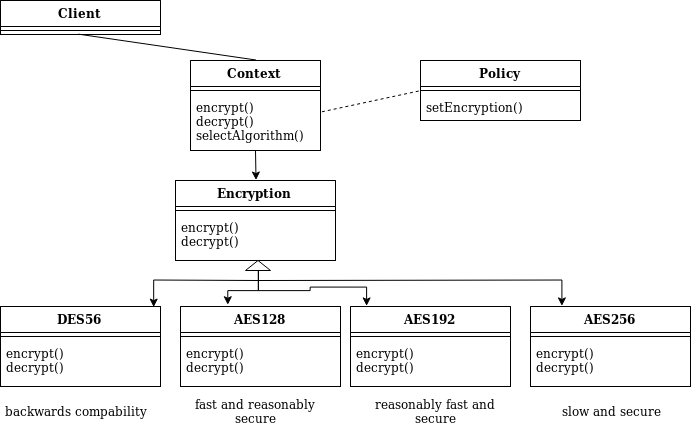
\includegraphics[width=15cm]{dg2.png}

In this model one uses the Strategy Pattern to model the different
encryption methods. The encryption method used is determined by the
setEncryption() method in the Policy class, using the DES algorithm
with 56 bit for legacy systems with necessary backwards compability, and
AES encryption of different strengths for different levels of security
and speed (systems with less secure encryption use smaller key sizes,
systems with bigger security requirements use longer key sizes).
Every encryption request is routed through a Context, which calls
the selectAlgorithm() method, which in turn uses the Policy class.

\section*{5}

Inheritance copies all methods and attributes from one class to a new
class and then extends this class (possibly overwriting existing methods
and attributes). It uses specified functionality from the parent class.
Delegation calls a method from a foreign class, it uses already
implemented functionality.

\end{document}
